\documentclass{beamer}
\usepackage{graphicx}
\usepackage{hyperref}
\usepackage{amsmath}
\usepackage{booktabs}
\usepackage{xcolor}

\begin{document}

\title{Predicting Supreme Court Case Outcomes}
\author{\textbf{Baraa Zekeria} \\ DSC 161: Text as Data}
\date{March 11, 2024}

\begin{frame}
\titlepage
\end{frame}


\begin{frame}{Research Question}
\begin{itemize}
    \item \textbf{Research Question:} \textit{Can we predict the outcome of Supreme Court cases using the opinions, concurrence, and dissent in the court's decisions?}
    \item \textcolor{blue}{Goal} $\Rightarrow$ Understanding if the \textbf{language} used in court opinions, concurrence, and dissent can predict case outcomes \textbf{has significant implications for legal practice and judicial decision-making}.
\end{itemize}

$$\text{win\_side} = f(\text{justia\_section})$$

\end{frame}


\begin{frame}{Data Source}
\begin{itemize}
    \item Data sourced from \href{https://aclanthology.org/2023.nllp-1.20/}{\textit{"Super-SCOTUS: A multi-sourced dataset for the Supreme Court of the US"}} by Biaoyan Fang et al.
    \begin{itemize}
        \item Aims to address complexity of US Supreme Court judiciary by integrating various procedural phases and resources.
        \item Provides a comprehensive dataset connecting language documents with extensive metadata.
    \end{itemize}
\end{itemize}
\end{frame}


\begin{frame}{Data Description}
\begin{itemize}
    \item Supreme Court cases from 2010 to 2015
        \begin{itemize}
            \item \textit{Why?} Justices are the same
            \item \begin{figure}
                  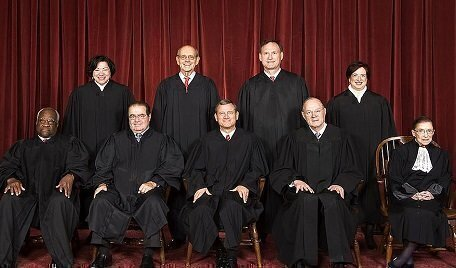
\includegraphics[width=0.5\textwidth]{img/roberts_court_2010.jpeg}
                  \caption{\textt{justia\_section} Word Cloud}
                  \end{figure}
        \end{itemize}
    \item The feature of interest is the \texttt{justia\_sections} variable, encompassing opinions, concurrences, and dissents.
\end{itemize}
\end{frame}


\begin{frame}{Data Cleaning and Text Preprocessing}
\begin{itemize}
    \item Parsed dictionary-like strings into dictionaries for relevant columns.
    \item Cleaned and preprocessed text data by removing stopwords, lemmatizing, and removing numbers.
\end{itemize}
\end{frame}


\begin{frame}{Modeling: TF-IDF Vectorization}
\begin{itemize}
    \item Split the dataset into training and testing sets using an 80-20 split.
    \item Applied TF-IDF vectorization to the textual content in \texttt{justia\_sections} (44K+ features)
\end{itemize}

\textbf{TF-IDF Formula:}
\[
\text{TF-IDF}(t, d, D) = \text{TF}(t, d) \times \text{IDF}(t, D)
\]
where:
\begin{itemize}
    \item $t$ represents a term (word) in the document
    \item $d$ represents a document
    \item $D$ represents the set of all documents
    \item $\text{TF}(t, d)$ is the term frequency of term $t$ in document $d$
    \item $\text{IDF}(t, D)$ is the inverse document frequency of term $t$ across all documents in $D$
\end{itemize}
\end{frame}


\begin{frame}{Modeling: TF-IDF Vectorization}
\begin{figure}
        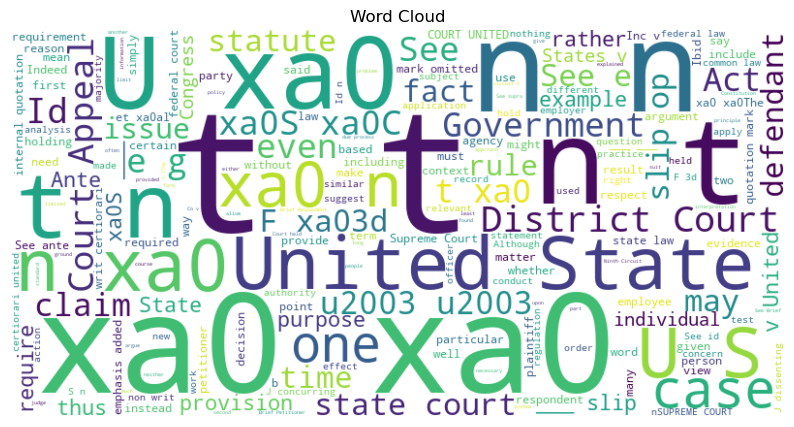
\includegraphics[width=0.8\textwidth]{img/word_cloud.png}
        \caption{\textt{justia\_section} Word Cloud}
\end{figure}
\end{frame}


\begin{frame}{Modeling: Classification}
\begin{itemize}
    \item Used \textbf{Naive Bayes} and \textbf{Logistic Regression} models for predicting the case outcomes based on the features extracted from \texttt{justia\_sections}.
\end{itemize}
\end{frame}


\begin{frame}{Results}
\begin{itemize}
    \item Utilized cross-validation to choose the best model, Logistic Regression   
        \begin{itemize}
            \item \textcolor{red}{Limitation of Naive Bayes}: \textit{naively} assumes each word is independent
        \end{itemize}
    \item Achieved an \textbf{accuracy of 62\%} on the test set with the best model.
    \item \begin{figure}
        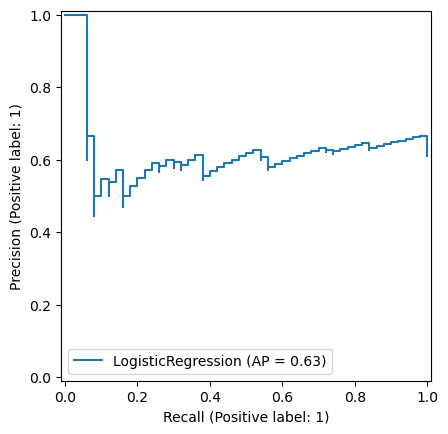
\includegraphics[width=0.5\textwidth]{img/logisitic_pr_curve.png}
        \caption{Logistic Regression Percision-Recall Curve}
    \end{figure}
\end{itemize}
\end{frame}

\begin{frame}{Limitations}
\begin{itemize}
    \item \textbf{Limited Feature Set}: reliance solely on textual content from \texttt{justia\_sections} may overlook valuable metadata
    \item \textbf{Data Imbalance}: imbalance between classes ("affirmed" vs. "reversed") impacted model performance
    \item \textbf{Simplified Models}: oversimplify complex relationships
        \begin{itemize}
            \item \textbf{Naive Bayes}: assumption of independence between words, leading to potential loss of context and meaning.
            \item \textbf{Logistic Regression}: linear decision boundaries may struggle to capture nonlinear relationships present in legal texts, limiting the model's ability to discern subtle patterns
        \end{itemize}
    \item \textbf{Bias and Fairness}: Risks of bias exist in the dataset and models, requiring careful mitigation for fair predictions.
    \item \textbf{Generalizability}: Model applicability beyond the dataset and timeframe needs validation for real-world use.
\end{itemize}
\end{frame}


\begin{frame}{Next Steps}
\begin{itemize}
    \item Possibly include additional features related to case metadata such as oral arguments, amicus briefs, petitioner, respondent, etc.
    \item Consider incorporating more advanced natural language processing techniques
\end{itemize}
\end{frame}

\end{document}
